\documentclass[11pt,a4j,fleqn]{jarticle}
\usepackage{amsmath,amsthm,amssymb}
\usepackage[dvipdfmx]{graphicx}
\usepackage{here}
\setlength{\textheight}{250mm}

%% \maketitleの余白を調整
\makeatletter
\renewcommand{\@maketitle}{\newpage
% \null
% \vskip 2em
\begin{center}
{\LARGE \@title \par} \vskip 1.5em {\large \lineskip .5em
\begin{tabular}[t]{c}\@author
\end{tabular}\par}
\vskip 1em {\large \@date} \end{center}
\par
\vskip 1.5em}
\makeatother

\title{作図プログラム}
\author{小川紗里奈}
\date{6/3}


\begin{document}

\maketitle

\section{はじめに}

わたし自身が包絡線定理の内容を理解していないので書けませんでした(泣)
数式などのコマンドはだいたいわかるので今後はなんとかなると思います、、

\section{包絡線定理}

適当に数式書いときます。
\[ F'(\alpha) = \frac{\partial f}{\partial \alpha}(x^*(\alpha), \alpha) \]

\begin{figure}[H]
 \centering
 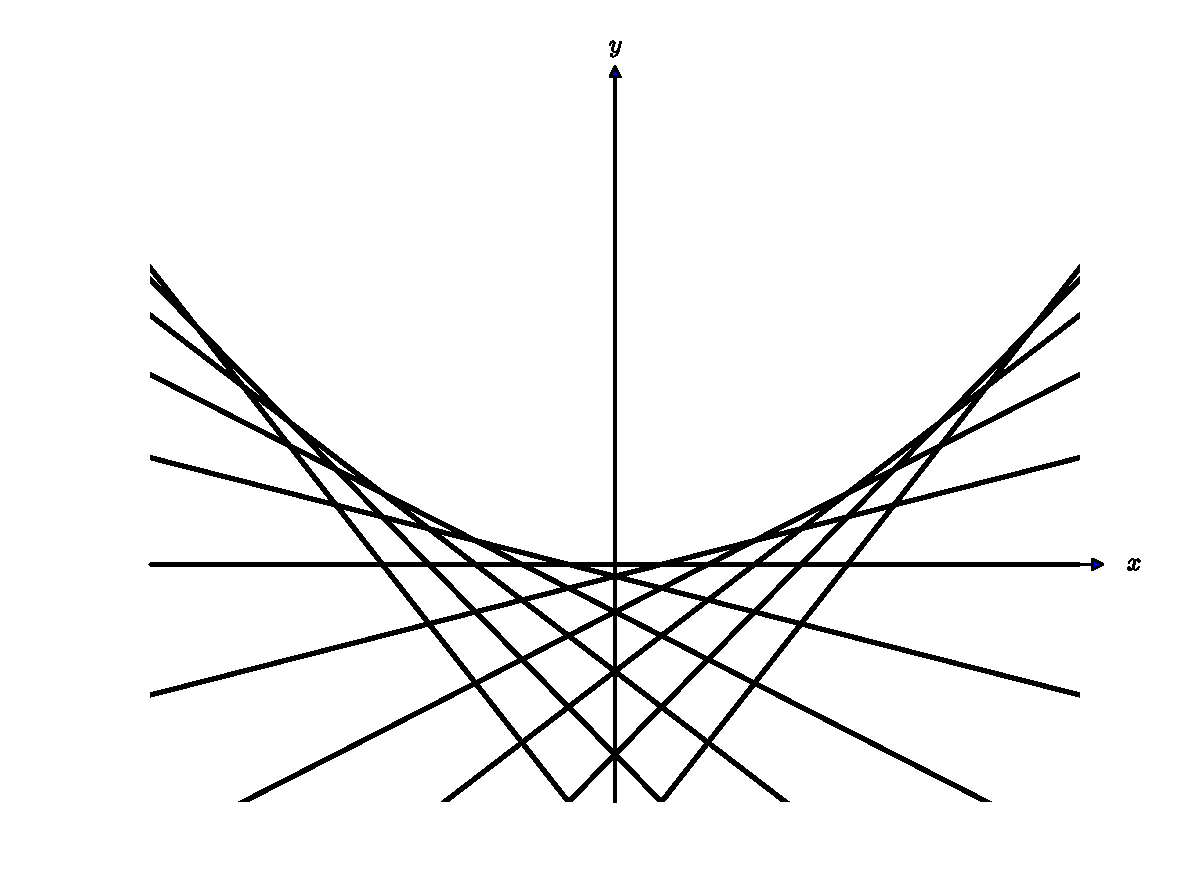
\includegraphics[width = 7cm]{envelope0.pdf}
 \caption{1つ目の図の表示}
 \label{fig:1}
\end{figure}

\begin{figure}[H]
 \centering
 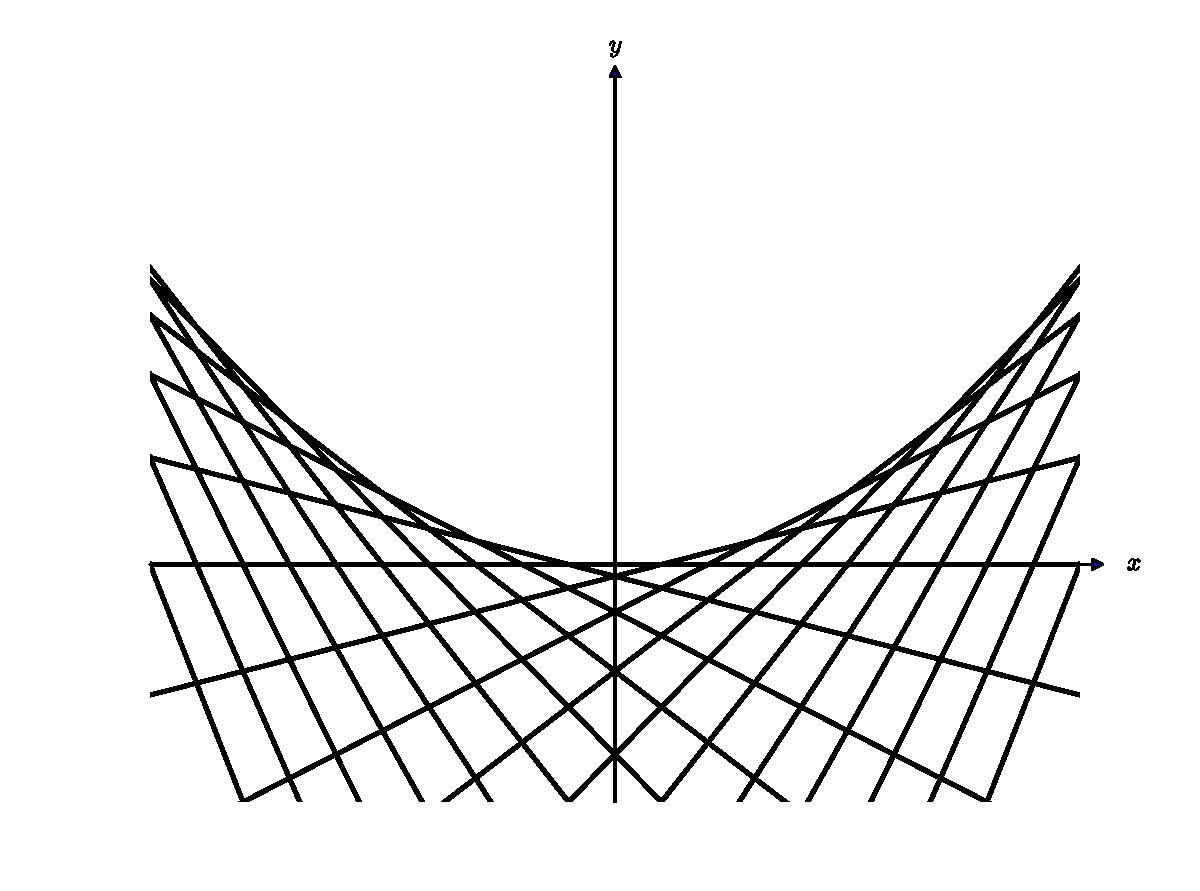
\includegraphics[width = 7cm]{envelope1.pdf}
 \caption{2つ目の図の表示}
 \label{fig:2}
\end{figure}



引用の例:尾山・安田\cite{OyamaYasuda11}

\section{Pythonプログラム}

\begin{quote}
\begin{verbatim}
from mpl_toolkits.axes_grid.axislines import SubplotZero
from matplotlib.transforms import BlendedGenericTransform
import matplotlib.pyplot as plt
import numpy as np

def f(x, t):
    return t * x - t**2

fig = plt.figure(1)
ax = SubplotZero(fig, 111)
fig.add_subplot(ax)

ax.axhline(linewidth=1.7, color="black")
ax.axvline(linewidth=1.7, color="black")

plt.xticks([])
plt.yticks([])
plt.ylim([-20,40])

ax.text(0, 1.05, '$y$', transform=BlendedGenericTransform(ax.transData,
 ax.transAxes), ha='center')
ax.text(1.05, 0, '$x$', transform=BlendedGenericTransform(ax.transAxes,
 ax.transData), va='center')

for direction in ["xzero", "yzero"]:
    ax.axis[direction].set_axisline_style("-|>")
    ax.axis[direction].set_visible(True)

for direction in ["left", "right", "bottom", "top"]:
    ax.axis[direction].set_visible(False)

x = np.linspace(-10, 10, 200)
for i in range(-5,6):
    y = f(x, t=i)
    ax.plot(x, y, 'black', linewidth=2)
plt.show()
\end{verbatim}
\end{quote}


\begin{thebibliography}{0}
\bibitem{OyamaYasuda11}
尾山大輔・安田洋祐「経済学で出る包絡線定理」『経済セミナー』2011年10・11月号.
\end{thebibliography}

\end{document}